%! Author = peter
%! Date = 9/20/2023

% Preamble
\documentclass[12pt,vi,twoside]{article}
\usepackage{subfiles}

% Packages
\usepackage{lgrind}
\usepackage{cmap}
\usepackage[T1]{fontenc}

\usepackage{microtype}
\usepackage{amsmath}
\let\Bbbk\relax
\usepackage{amssymb}
\usepackage{gensymb}
\usepackage{graphicx}
\usepackage{pgf}
\usepackage{float}
\usepackage{optidef}
\usepackage{ifdraft}
\usepackage[hyphens]{url}
\usepackage{hyperref}
\usepackage{enumitem}

\renewcommand{\labelitemii}{$\circ$}

\usepackage{eqexpl}
\eqexplSetIntro{where:} % set parenthesis in the left of the first item
\eqexplSetDelim{=} % set delimiter to "="

\usepackage{ar}

\usepackage{multicol}

\usepackage{siunitx}
\sisetup{}

\usepackage{tabularx}
\usepackage{booktabs}
\usepackage{multirow}
\usepackage{tablefootnote}
\usepackage{tabularray}
\UseTblrLibrary{booktabs}

\usepackage{mdframed}
\newmdenv[
    topline=false,
    bottomline=false,
    skipabove=\topsep,
    skipbelow=\topsep,
    innerleftmargin=30pt,
    innerrightmargin=30pt,
    backgroundcolor=black!5
]{example}

\usepackage{fontspec}
\setmonofont{Source Code Pro}
\setmainfont{TeX Gyre Pagella}
%\setmainfont{Fira Sans}
%\setmainfont{TeX Gyre Heros}

\usepackage{tikz}
\usetikzlibrary{positioning}
\usetikzlibrary{shapes.geometric}
\usetikzlibrary{shapes.arrows}
\usetikzlibrary{decorations.pathmorphing, decorations.pathreplacing, calc}

\usepackage{tikz-cd}
\tikzcdset{
    math mode=false
}

\usepackage[outputdir=../out,final=true]{minted}
\PassOptionsToPackage{table,xcdraw}{xcolor}
\usepackage{xcolor}

\definecolor{c1}{HTML}{64ACBE}
\definecolor{c2}{HTML}{EE442F}
\definecolor{c3}{HTML}{601A4A}

\definecolor{myorange}{RGB}{255, 165, 0}
\definecolor{mydarkseagreen}{RGB}{143, 188, 143}
\definecolor{mydodgerblue}{RGB}{30, 144, 255}

\colorlet{b}{red!13!white}
\colorlet{m}{yellow!20!white}
\colorlet{g}{green!18!white}


\renewcommand{\theFancyVerbLine}{\sffamily
    \textcolor[rgb]{0.8,0.8,0.8}{\scriptsize\oldstylenums{\arabic{FancyVerbLine}}}
}
\usemintedstyle{pastie}
%\usemintedstyle{jupyter_python}
%\usemintedstyle{rainbow_dash}
%\usemintedstyle{colorful}
\setminted{
    frame=lines,
    framesep=2mm,
%    numbers=left,
    fontsize=\footnotesize,
    autogobble=true,
    baselinestretch=1.15,
    breaklines
}
\setmintedinline{
    breaklines
}

\usepackage{titlesec}
%\newcommand{\sectionbreak}{\clearpage}

\usepackage{enumitem}

\usepackage{caption}
\captionsetup[table]{skip=6pt}

\usepackage[numbers,sort&compress]{natbib}

\usepackage{adjustbox}

\usepackage[titletoc,title]{appendix}

\usepackage{geometry}
\geometry{
    letterpaper,
    left=1.0in,
    right=1.0in,
    top=1.0in,
    bottom=1.0in
}

\usepackage{setspace}
\setstretch{1.5}

\usepackage{svg}

\usepackage{subcaption}

\usepackage{afterpage}
\usepackage[section]{placeins}

\usepackage{nth}

% Matrices and vectors
\newcommand{\mat}[1]{
    \mathbf{#1}
}

% Derivatives and Partials
\newcommand{\pdiff}[2]{
    \frac{\partial #1}{\partial #2}
}
\newcommand{\pddiff}[2]{
    \frac{\partial^2 #1}{\partial #2^2}
}
\newcommand{\pddiffm}[3]{
    \frac{\partial^2 #1}{\partial #2 \partial #3}
}

\newcommand{\diff}[2]{
    \frac{\mathrm{d} #1}{\mathrm{d} #2}
}
\newcommand{\ddiff}[2]{
    \frac{\mathrm{d}^2 #1}{\mathrm{d} #2^2}
}
\newcommand{\ddiffm}[3]{
    \frac{\mathrm{d}^2 #1}{\mathrm{d} #2 \mathrm{d} #3}
}

% Sets
\newcommand{\R}[0]{
    \mathbb{R}
}
\newcommand{\Z}[0]{
    \mathbb{Z}
}

% Orders
\newcommand{\order}[0]{
    \mathcal{O}
}


\newcommand{\Rey}{\rm Re}
\newcommand{\M}{\rm M}
\newcommand{\Cp}{C_p}
\newcommand{\Cpo}{C_{p_0}}
\newcommand{\Cpm}{C_{p_{\rm min}}}
\newcommand{\Cpom}{C_{p_{0,\rm min}}}
\newcommand{\Cpcr}{C_{p_{\rm crit}}}
\newcommand{\Mcr}{M_{\rm crit}}
\newcommand{\Mdd}{M_{\rm dd}}
\newcommand{\Mi}{M_\infty}
\newcommand{\Ncr}{N_{\rm crit}}


\title{PhD Proposal Document}
\author{Peter Sharpe}
% Document
\begin{document}

    \begin{center}

        \vspace*{1cm}

        \textsc{Massachusetts Institute of Technology}

        Department of Aeronautics and Astronautics

        \vspace{1cm}

        \textbf{PhD Proposal Document}

        \vspace{1cm}

        \textbf{\large Advancing the Usability, Interpretability, and Practicality of Conceptual Aircraft Design Optimization with Code Transformations}
        \vspace{1cm}

        \textit{Ph.D. Candidate:}\\
        Peter Sharpe

        \vspace{1cm}

        \textit{Committee:}\\
        Professor R. John Hansman (Chair), MIT\\
        Professor Mark Drela, MIT\\
        Professor Karen Willcox, University of Texas at Austin\\

        \vspace{1cm}

        \textit{External Evaluator:}\\
        Dr. Tony Tao, MIT Lincoln Laboratory

        \vspace{3cm}

        December 11, 2023

    \end{center}

%    \clearpage
    \section*{Abstract}

    TODO abstract

%    \clearpage

    % table of contents
    \tableofcontents


    \section{Introduction}

    \subsection{Background}

    TODO intro

    \subsection{Project Definition and Thesis Overview}

    \subsection{Motivation for Improving Industry Access to Design Optimization}

    \subsection{Document Organization}

    The latest doctoral handbook for the MIT Department of Aeronautics and Astronautics requires the following elements in a PhD proposal, which, for reader convenience, are mapped to specific portions of this document:

    \begingroup
    \renewcommand{\arraystretch}{1.5} % Default value: 1
    \begin{table}[H]
        \centering
        \caption{Requirement-to-section mapping for the PhD proposal document.}
        \label{tab:toc}
        \begin{tabular}{p{10cm}|p{4cm}}
            Requirement                                                                                      & Section                                             \\
            \hline
            A clear, specific statement of the technical problem and the objectives of the proposed research & Section \ref{sec:intro}, \ref{sec:technical-gap} \\
            A thorough, adequately referenced, summary of previous work done on the problem                  & Section \ref{sec:literature}                        \\
            A plan for the initial approach to the problem                                                   & Section \ref{sec:contributions}                     \\
            An outline of the major foreseeable steps to a solution of the problem                           & Section \ref{sec:contributions}, \ref{sec:schedule} \\
            An estimate of the time that might be required                                                   & Section \ref{sec:schedule}                          \\
            A list of the facilities needed                                                                  & Section \ref{sec:facilities}                        \\
        \end{tabular}
    \end{table}
    \endgroup


    \section{A Review of Aircraft Design Optimization}
    \label{sec:literature}

    \subsection{Early Promises, Predictions, and Pitfalls}

    \begin{quote}
        \textit{``When an aircraft designer hears that a new program will use multidisciplinary optimization, the reaction is often less than enthusiastic. Over the past 30 years, aircraft optimization at the conceptual and preliminary design levels has often yielded results that were either not believable, or might have been obtained more simply using methods familiar to the engineers. Even 5-20 years ago, actual industry application of numerical optimization for aircraft preliminary design was not widespread.''}
        \flushright-Ilan Kroo, 1997 \cite{kroo_multidisciplinary_1997}
    \end{quote}

    These are the opening lines of a landmark 1997 paper that reviewed the state of the art and future directions in the then-nascent field of aircraft multidisciplinary design optimization (MDO) \cite{kroo_multidisciplinary_1997}. The paper, by aircraft designer and MDO pioneer Ilan Kroo, not only reviewed the status of the field's academic research, but also took the key step of assessing whether these research advances had translated to practical industry impact. As a later review by an MDO technical organizing committee would emphasize, ``the ultimate benchmark of a research field's impact is indicated by the realization of its theories into successful products throughout industry.'' \cite{agte_mdo_2010}

    Kroo's assessment of the field is generally optimistic, but with some important reservations. On one hand, he notes the auspicious progress of aircraft MDO research during the preceding decades by all traditional metrics: problem size, analysis fidelity, runtime speed, and so on. He credits these successes largely to both algorithmic advances and the exponential growth of computational power over time (Moore's law\footnote{``Moore's law'' is an empirical observation that chip transistor density (a surrogate for computational power) has tended to double roughly every two years, a trend that has held true for the past half-century.}). Extrapolating these trends forward, he concludes that the field is poised to make a significant impact on the aircraft design process across both academia and industry. The promise of MDO is made clear in a remark that many aircraft designers would agree with today: ``In a very real sense, preliminary design is MDO.'' \cite{kroo_multidisciplinary_1997}

    On the other hand, Kroo notes that actual industry applications of aircraft MDO remained conspicuously limited as of the paper's 1997 publication, and ``many difficulties remain in the routine application of MDO.'' \cite{kroo_multidisciplinary_1997} Other works from the early days of aircraft MDO corroborate this dearth of industry adoption. For example, in a 1982 AIAA lecture titled \textit{On Making Things the Best -- Aeronautical Uses of Optimization}, optimization advocate Holt Ashley notes the ``keen disappointment felt by many [optimization] specialists because their theories have received so little practical application.'' \cite{ashley_making_1982} Ashley goes further by conducting an exhaustive industry-wide survey to identify ``successful practical applications'' of aircraft design optimization. The survey received ``overwhelming'' industry interest and encouragement; however, ``the yield of examples which met the criterion of having been incorporated into a vehicle that actually operates in the Earth's atmosphere was painfully, perhaps shockingly small.''

    Perhaps the reason for Ashley's pain is that, even at the time, aircraft designers in industry widely recognized the immense potential of MDO tools to fundamentally transform engineering design workflows. As two Lockheed engineers stated in 1998 \cite{radovcich_f22_1998}, ``The technical community knows the power of MDO and not having a cradle-to-grave example has been a continual source of frustration, as voiced by AIAA MDO technical committee members [for] years.'' Similarly, a 2002 Boeing paper identifies MDO as one of four key technologies poised to define the next generation of aircraft design\footnote{With the others being computational simulation, small uncrewed aircraft, and newly-emphasized design considerations such as environmental footprint and operations optimization.} \cite{mcmasters_airplane_2002}.

    Motivated by this gap between promise and practice, Kroo and other luminaries offer several reasons for the lack of industry adoption of MDO technologies:

    \begin{enumerate}
        \item \textbf{Inadvertently-violated model assumptions:} When optimization is applied to an analysis toolchain, it acts adversarially, disproportionately seeking out the ``weakest link'' in the analysis chain and exploiting it. Simplified models that are acceptable in a manual sizing study are often unacceptable in an optimization study, because implied assumptions that an engineer would naturally cross-check during manual design are prone to optimizer exploitation. This can lead to unrealistic results from MDO tools that degrade user trust in optimization processes. Kroo contends that the solution to this problem is to implement higher-fidelity models that account for more edge cases, an approach we explore later in Section \ref{sec:wide_vs_deep}.
        \item \textbf{Missing models and constraints:} Critical aircraft design choices are often determined by tradeoffs spanning multiple disciplines. If an MDO tool does not incorporate relevant disciplines (e.g., it performs aerodynamic, propulsive, and structural analyses, but the true design driver is noise), then the resulting design will be fundamentally flawed with no indication to the user whatsoever. This can lead to costly design mistakes. Indeed, Kroo suggests that a flawed MDO tool is not only useless, but worse, due to the false confidence it can instill.
        \item \textbf{Challenges of managing complexity:} As computational power grows, MDO tools can incorporate increasingly numerous and higher-fidelity models. To first order, when the number of models $N$ grows, the potential number of cross-discipline couplings to manage tends to scale as $\mathcal{O}(N^2)$. Therefore, in the limit of growing computational power, the practical bottleneck is less about implementing individual analyses, but more about managing this communication overhead and architecting the optimization code itself.
    \end{enumerate}

    Kroo primarily attributes these early barriers to practical industry adoption to the limited computational power of the era, noting: ``This convergence between computational capability and computational requirements for interesting design problems is one of the reasons that MDO is considered to be such a promising technology, despite the limited acceptance of pioneering MDO efforts.'' A contemporaneous review by Sobieski and Haftka agreed, identifying ``very high computational demands'' as a ``major [obstacle] to realizing the full potential of MDO''. \cite{haftka_multidisciplinary_1997}

    However, some works recognized that not all challenges would recede with increasing computational power. A 2002 review paper by a Boeing Technical Fellow in \textit{Journal of Aircraft} \cite{mcmasters_airplane_2002} cautions: ``New [MDO] strategies need to be developed\dots which take advantage of the assumptions and techniques that airplane designers use, rather than letting a computer churn away and come up with theoretically possible, but practically impossible, configurations.'' Likewise, Kroo, Sobeiski, and Haftka all cite ``managing complexity'' as a growing challenge of MDO \cite{kroo_multidisciplinary_1997, haftka_multidisciplinary_1997}. Drela's aptly-titled 1998 work \textit{Pros \& Cons of Airfoil Optimization} also demonstrates a similar issue \cite{drela_pros_1998}. Here, Drela demonstrates that even seemingly-simple design optimization problems will only yield practical results if the problem formulation, assumptions, and results are all precisely understood by an expert designer. These works presciently foreshadow modern concerns around MDO interpretability and other user frictions, urging the development of human-centered MDO approaches that synthesize mathematical optimization with designer intuition.

    In summary, while computational limits were a clear early barrier, foundational challenges around managing complexity and aligning optimization with real-world design constraints were already emerging. These issues would become increasingly central as MDO research rapidly expanded in scope.

    \subsection{A Retrospective on Aircraft Design Optimization in Industry}

    \subsubsection*{Current Status}

    With the benefit of an additional quarter-century of hindsight since the date of these early MDO assessments, we can begin to assess how these forecasts have played out. In many ways, these predictions by Kroo and others were remarkably accurate. The scale and speed of optimization problems solved today has indeed grown exponentially in the years since. This is not only due to increasing computational power, but also from algorithmic and architectural improvements in MDO and optimization more broadly\footnote{discussed later in Section \ref{sec:literature_advances}}. Numerous high-quality aircraft MDO case studies and post-hoc design studies have been published in the years since, including the D8 transport aircraft \cite{drela_development_2011, drela_tasopt_2010}, the STARC-ABL aircraft \cite{yildirim_performance_2021}, and the Aerion AS2 \cite{bons_highfidelity_2020}. Some of these studies leverage relatively-high-fidelity models (e.g., RANS CFD) that would have been computationally-intractable for optimization studies in prior eras.

    However, many of the barriers to practical industry use Kroo identified have not disappeared; to the contrary, as computational power increases, the challenges of interpretability and managing complexity ring even truer today. As a result, this gap between academic research and practical industry adoption has not closed, and in some ways is wider than ever before. A 2010 review paper \cite{agte_mdo_2010} concludes that ``the actual use of genuine MDO methods within industry at large\dots is still rather limited.'' In 2013, Hoburg and Abbeel lamented that ``despite remarkable progress in MDO, the complexity and diversity of modern aerospace design tools and teams makes fully coordinated system-level optimization a monumental undertaking.'' \cite{hoburg_geometric_2014} As recently as 2017, a team of Airbus engineers and MDO researchers concurred: ``While the field of MDO techniques has tremendously grown since [the 1980s] in the scientific community, its application in industry is still often limited[\dots]\ A major challenge remains to apply MDO techniques to industrial design processes.'' \cite{gazaix_industrialization_2017}

%     The field has also seen the development of several general-purpose MDO frameworks, including OpenMDAO \cite{gray_openmdao_2019}, GPKit \cite{gpkit}, and AeroSandbox \cite{sharpe_aerosandbox_2021}.

    Despite the prevalence of on-paper design studies using MDO, it remains somewhat rare to see \textit{built-and-flown} airplanes developed with documented, significant use of MDO methodologies. Indeed, the industry norm for aircraft conceptual design remains largely unchanged: expert-driven manual design guided primarily by point analyses and parametric surveys. Here, the human designer informally fulfills an optimizer-like role, but the requirements are never explicitly translated into a formal mathematical optimization problem\footnote{i.e., with a precisely specified objective, defined variables, and enumerated constraints}. High-quality aircraft design case studies that implement this expert-driven manual approach successfully are those of the Joby Aviation S2 eVTOL \cite{stoll_conceptual_2014} and Perdix micro-UAV \cite{tao_design_2012} aircraft. Anecdotally, the industry conceptual designer's computational weapon of choice is still more often an Excel spreadsheet than a formalized MDO framework.

    To quantify this gulf between academic and industry use of MDO, we surveyed industry literature and design reviews to identify aircraft development programs showing three minimal criteria:
    \begin{enumerate}[noitemsep]
        \item A design optimization problem for a complete aircraft coupling at least three disciplines (e.g., aerodynamics, structures, and propulsion) that is solved computationally.
        \item Evidence that the optimization result (or at least, some insight gained from it) was used to inform the design of aircraft.
        \item Evidence that the aircraft was subsequently built and flown.
    \end{enumerate}

    \noindent It is worth pausing to discuss why this restrictive \textit{built-and-flown} aircraft requirement is used, since it accounts for the majority of the aircraft design studies that were excluded from this survey. Successful optimization on built-and-flown aircraft forces a level of completeness, trust, and durability that may not be present in a paper study. Ashley notes that a practical MDO result ``must also survive the gauntlet of ground testing, reliability, demonstration, flight verification, and the like without further special attention''. \cite{ashley_making_1982} Myriad other practical considerations could be added to this list -- certifiability, manufacturability, lifecycle costs, maintainability, robust off-design performance, and the realities of engineering culture (e.g., can the MDO tool give not only a result, but sufficient evidence that it should be believed?), to name only a few. To justify the substantial capital of building and flying a new aircraft, optimization results must withstand a much higher standard of scrutiny and reviewability than they might otherwise.

%    We find that relatively few programs meet these criteria. This is broadly consistent with previous surveys and reviews \cite{kroo_multidisciplinary_1997, agte_mdo_2010, ashley_making_1982, haftka_multidisciplinary_1997,gazaix_industrialization_2017}, although

    Consistent with previous surveys and reviews \cite{kroo_multidisciplinary_1997, agte_mdo_2010, ashley_making_1982, haftka_multidisciplinary_1997,gazaix_industrialization_2017}, we find that relatively few programs meet these criteria; here, we make note of some that do. The Lockheed Martin F-22 Raptor program was one of the first programs to leverage an MDO-like process for a complete, flown aircraft design, as reported by Radovcich and Layton \cite{radovcich_f22_1998}. However, the workflow documented in this 1998 work differs significantly from modern MDO processes in that it was remarkably manual -- a fusion of traditional and MDO-based design processes. While some disciplines (aerodynamics, structures, and control law design) are coupled computationally, many other disciplines (low-observability, manufacturability, etc.) are coupled in by querying teams of subject-matter experts at iterates within the optimization loop itself, essentially serving as a black-box function call. When contrasted with more-typical MDO processes where all interdisciplinary communication is computational, this manual approach has some pros and cons. One one hand, intermediate optimization iterates are continuously human-reviewed, potentially boosting trust. On the other hand, it also sharply increases the optimization runtime, from hours to months. Even allowing for this broader definition of MDO, however, the authors note the rarity of their experience in industry: ``Documented experiences of MDO applications during the engineering, manufacturing, and design phases of fighter aircraft programs are not numerous. Documentation is even rarer for aircraft that have flown.''

    The Lockheed Martin X-59 Quiet Supersonic Transport (QueSST) is another program that leveraged an MDO-based design process throughout aircraft development, unifying aerodynamics, acoustics, and structural analyses for outer mold line design and composite ply scheduling \cite{x59_nasa_nas, x59_nasa_sc19, x59_compositeworld}. (Although the X-59 has not yet met the ``flown'' criterion at the time of writing, industry reports credibly suggest this is imminent with no remaining obvious barriers.) The X-59 program builds upon several decades of successful MDO research for sonic-boom-minimization problems, a topic where computational shape optimization has proven particularly useful due to the non-intuitive and sensitive nature of the design problem \cite{choi_multifidelity_2008}.

    The Airbus \textit{Vahana}, a single-seat eVTOL demonstrator flown in 2018, is perhaps one of the most recent public examples of an MDO-based process used to develop a flown aircraft \cite{vahana_1, vahana_2, vahana_code}. The initial sizing study considered aerodynamics, structures, propulsion, and cost analysis to drive conceptual trade studies between various vehicle configurations. Practical constraints and margins, such as reserve mission energy, battery cycle life, and engine-out safety (by enforcing either autorotation capability, motor redundancy, or a mass allocation for a ballistic parachute, depending on configuration), were included.

    Several other programs have built and flown uncrewed research aircraft with MDO use, such as the Facebook \textit{Aquila} solar-powered UAV \cite{fbhale}, the MIT \textit{Jungle Hawk Owl} long-endurance UAV \cite{jho}, and the X-48B blended-wing-body demonstrator \cite{wakayama_2000_blended, liebeck_blendedwingbody_1998, liebeck2004design}. Other programs document MDO usage for narrower subsystem- or component-level design, as in the detailed design of the Boeing 787 Dreamliner \cite{agte_mdo_2010}.

    Aside from this, documented industrial use of MDO for complete-aircraft design remains relatively uncommon, especially in light of its widely-recognized potential utility. This lack of use can be partially explained as a lag effect stemming from long timelines of new aircraft development programs; it takes time for new tools to proliferate due to sunk-costs on design pipelines for existing programs. Indeed, the present literature review finds that documented industry use of MDO, while still uncommon, appears somewhat less scarce than previous surveys indicate \cite{kroo_multidisciplinary_1997, agte_mdo_2010, ashley_making_1982, haftka_multidisciplinary_1997, gazaix_industrialization_2017}; this suggests that industry use may be gradually increasing. However, as aircraft MDO research and substantial industry interest in optimization dates back roughly forty years \cite{vanderplaats_automated_1976, ashley_making_1982}, this lag effect alone does not constitute a complete explanation.

    Ashley considers another possible explanation for the lack of visible MDO use in industry: that of ``military classification or company proprietary considerations.'' \cite{ashley_making_1982} However, after exhaustive correspondence with dozens of aircraft design industry contacts, Ashley concludes that this limitation was only occasional and ``not to an extent that would affect the principal conclusions.'' Even after decades, industry usage of formal mathematical optimization processes for aircraft design remains fairly limited, and, when used, often leverages only a small fraction of the field's research advances.

    \subsection{Pivotal Advances in Design Optimization Research}
    \label{sec:literature_advances}

    On a more optimistic note, MDO's substantial academia-industry gap is equally attributable to academia's remarkable advances in design optimization research over recent decades. This progress is readily apparent from analyzing trends in academic literature. As shown in Figure \ref{fig:mdo_citation_counts}, the fraction of aircraft design publications directly referencing MDO has grown from near-zero in 1985 to 10\% today.

    However, this statistic alone understates the true magnitude of MDO's impact. Arguably the most pivotal contribution of MDO research to aircraft design has been to catalyze a shift towards an \textit{optimization mindset}: the recognition that optimization is not only a useful tool, but also a principled mathematical framework that can represent complete design problems. Figure \ref{fig:mdo_citation_counts} shows that this mindset is a relatively recent development -- the fraction of aircraft design publications mentioning optimization in any form has tripled since the advent of MDO, reaching a majority share today.

    \begin{figure}[h]
        \centering
        \ifdraft{}{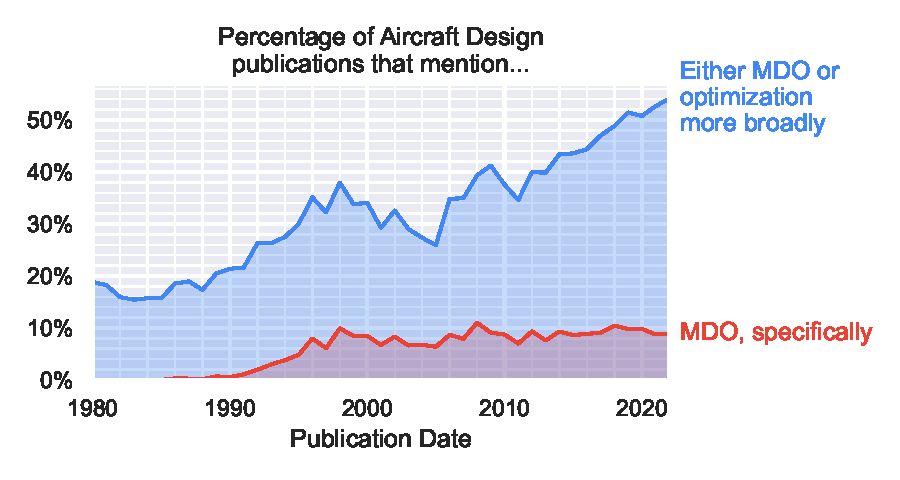
\includegraphics{../figures/mdo_citation_counts}}
        \caption{Prevalance of optimization-related keywords in academic literature with the keyword ``aircraft design''. Data from Google Scholar; includes industry-standard texts such as AIAA journals and conference proceedings. MDO-specific keywords (red line) include any of: ``multidisciplinary design optimization'', ``MDO'', and ``MDAO''. Blue line adds the keyword ``optimization'' to this list.}
        \label{fig:mdo_citation_counts}
    \end{figure}

    These optimization-based design processes have shown several benefits when used to augment traditional design methods such as point analyses, parametric surveys, and carpet plots \cite{torenbeek_advanced_2013}. Most obviously, formal optimization methods can lead to improved design results and allow the consideration of many more design variables. Optimization can also help human designers discover clever cross-discipline synergies that might otherwise be overlooked \cite{drela_pros_1998}, and its rigor can reduce the likelihood of biased decisions \cite{torenbeek_advanced_2013}. In cases where designer intuition is exhausted, such as with unconventional configurations, optimization provides a means to identifying useful directions for further exploration \cite{drela_pros_1998}. Torenbeek argues that an optimization-based design process can respond more quickly to unexpected changes in program requirements, whereas manual processes often require substantial redesign effort \cite{torenbeek_advanced_2013}. Finally, even the exercise of translating given requirements into a quantified optimization problem can prove useful -- this can help a team of designers align on goals and expose subtle discrepancies in perceived requirements\footnote{For example, is the objective to minimize fuel burn, or to maximize range? Is operating cost a quantity that should be strictly capped (a constraint), or instead only penalized (an objective)?}.

    Another important area where MDO research has made significant progress is in defining the relationship between the human designer and the optimizer. Several early aircraft design optimization works from the 1970s, with titles such as ``Automating the Design Process'' \cite{heldenfels_automating_1973, heldenfels_automation_1974, vanderplaats_automated_1976}, speculated that optimization would eventually advance to the point that computational tools could yield complete, production-ready designs with minimal human oversight. Over time, this has largely given way to a more balanced view: although the optimization solve itself may be well-served by computational means, this forms only one small part of the larger design process. Inputting the engineer's design intent into the optimizer accurately (``problem specification'') and extracting intuition from the results (``interpretation'') are challenges in their own right, and best addressed by iterative human-computer teams. As described by Drela in 1998 optimization study \cite{drela_pros_1998}, ``[Engineering optimization] is still an iterative cut-and-try undertaking. But compared to [traditional] techniques, the cutting-and-trying is not on the geometry, but rather on the precise formulation of the optimization problem.''

    When considering this full design process (i.e., from initial requirements to product delivery), the scope of challenges becomes even broader. Indeed, industry adoption of MDO is often limited by non-computational user frictions \cite{salas_framework_1998, gpkit, martins_engineering_2021}. In the present work, we deliberately term these user frictions ``costs'', borrowing optimization nomenclature to emphasize that minimizing these frictions is an implied part of the objective function of any optimization-driven design process.

    Figure \ref{fig:birds_eye_view} summarizes a variety of design literature to present a holistic view of this complete process as applied to aircraft design \cite{torenbeek_advanced_2013, martins_engineering_2021, yang_observations_2009, torenbeek_synthesis_1976, roskam_airplane_1989, nicolai_fundamentals_2010, salas_framework_1998}. Frictions that a designer may experience from a computational optimization framework at each step are shown in \textcolor[HTML]{BB5045}{red}.

    \begin{figure}[H]
        \centering
        \ifdraft{}{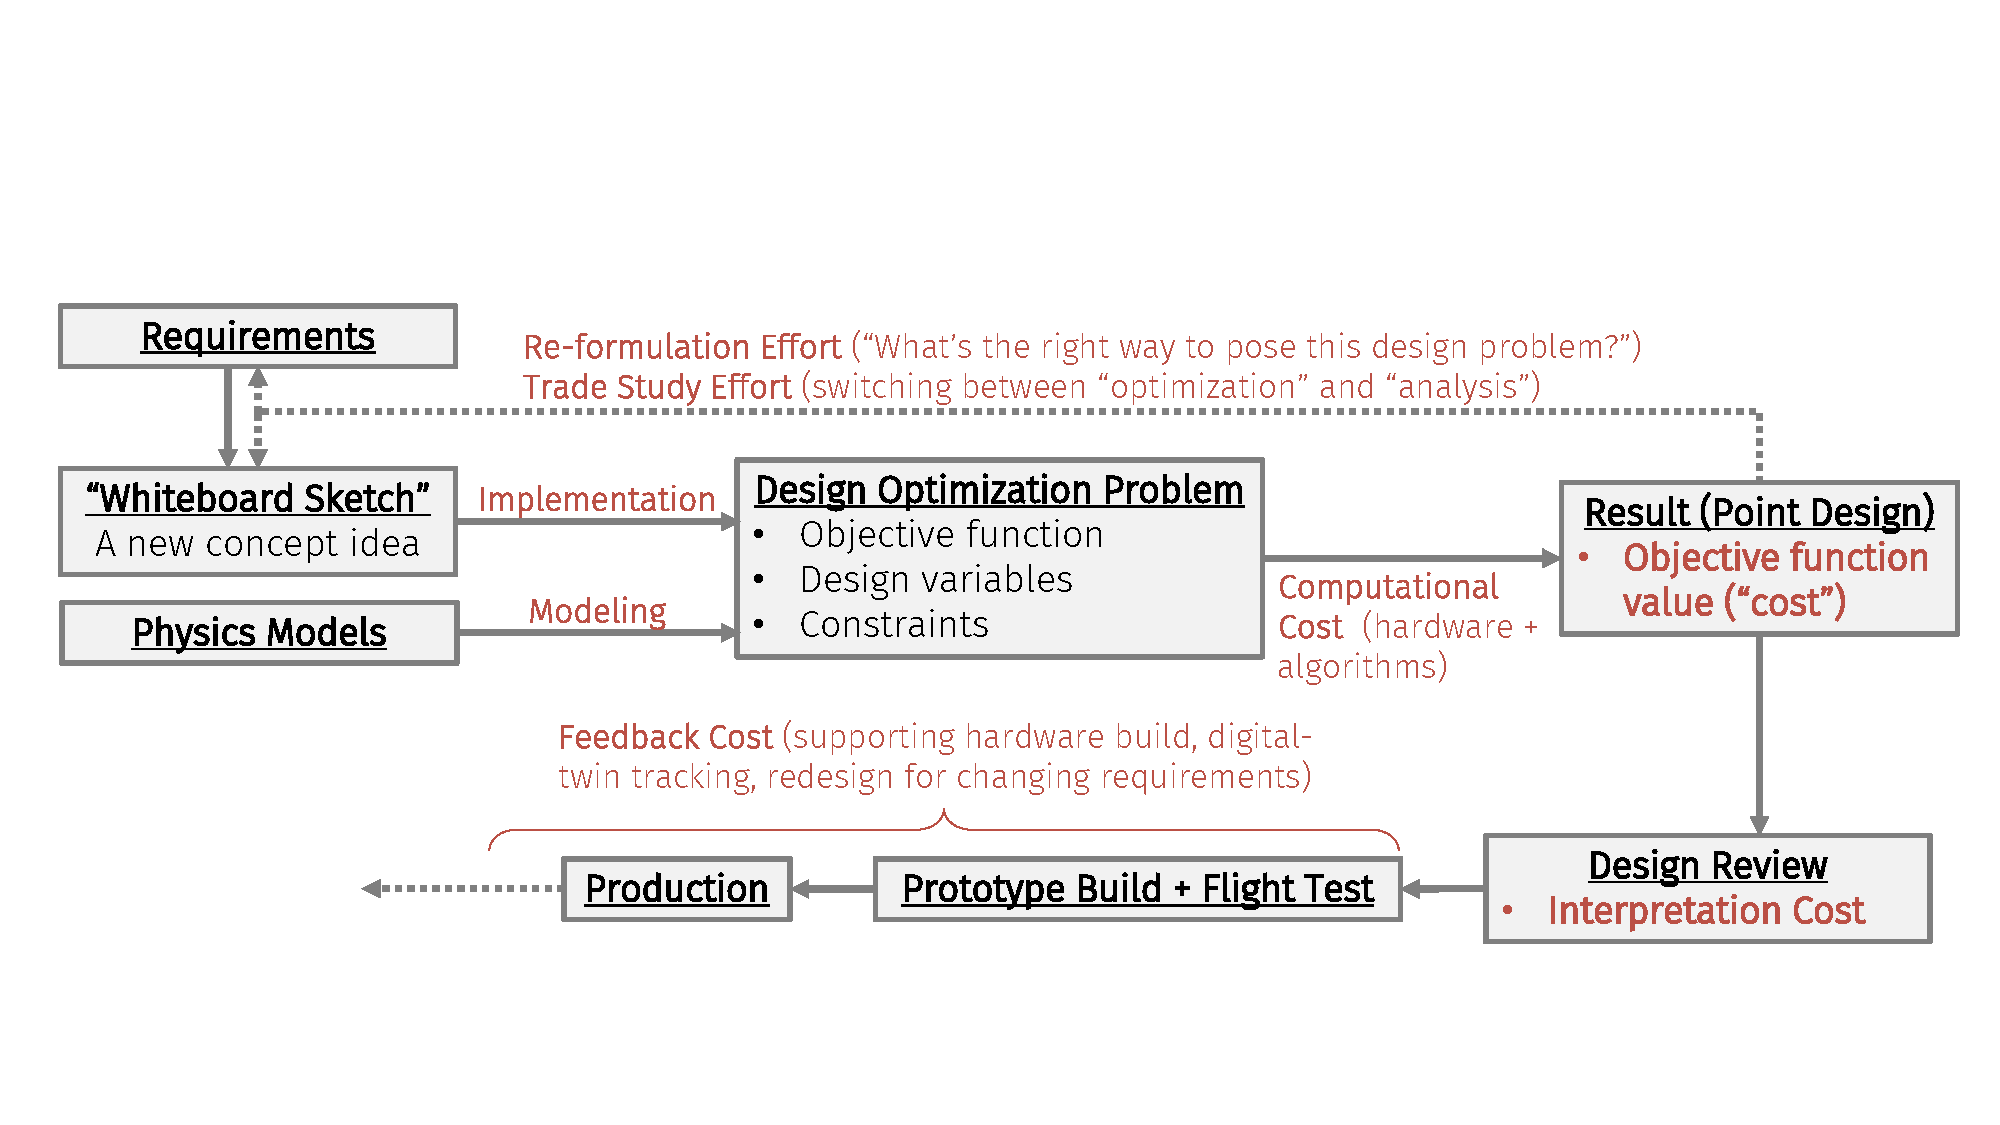
\includegraphics[width=\textwidth]{../figures/design_optimization_process_birds_eye_view}}
        \caption{A high-level overview of the optimization-driven design process, as applied to aircraft design. ``Costs'' (user frictions to be minimized) associated with each step are shown in \textcolor[HTML]{BB5045}{red}.} % says red, but hex code BB5045
        \label{fig:birds_eye_view}
    \end{figure}

    In the aircraft design process model of Figure \ref{fig:birds_eye_view}, the initial point of departure is a set of high-level requirements \cite{torenbeek_synthesis_1976, torenbeek_advanced_2013}. The first design step is to develop a set of candidate concepts (``sketches''), a qualitative process that largely leverages designer creativity and experience \cite{yang_observations_2009, roskam_airplane_1989}. Concepts and the associated requirements are then translated into a design optimization problem consisting of an objective function, design variables, and constraints. % TODO continue

    The remainder of this section will discuss some of the most important advances in design optimization research that have helped to reduce the costs incurred at various steps of this holistic process.

    \subsubsection{Two Directions: ``Wide'' vs. ``Deep'' MDO}
    \label{sec:wide_vs_deep}

    \subsubsection{Advances in Optimization Algorithms}

    \subsubsection{Advances in Design Optimization Practice}
%     complexity -- motivating the idea of general-purpose \textit{MDO frameworks} to address this as opposed to problem-specific codes

    % Multipoint

    % UQ


    % Importance of geometry - CPACS, Haimes work


    A notable area where computational methods for aircraft design have long made inroads to industry is in inverse design tools. (As an aerodynamic example, the inverse approach used by the XFoil airfoil design code \cite{drela_xfoil_1989} and others \cite{liebeck_blendedwingbody_1998} to recover a shape from a specified pressure distribution.) These tools can be seen as an alternative workflow to optimization approaches\footnote{Interestingly, inverse design tools can be viewed mathematically as a subset of nonlinear optimization, where the feasible space is a single point and there is no objective function.}, in that they aim to create a mapping from ``performance specification space'' back to the ``design space''. Drela \cite{drela_pros_1998} and others

    \subsubsection{Emerging Trends and Opportunities}


    It would be remiss to discuss the last decade of optimization advances (and in particular, the growing recognition of the \textit{interpretability problem} of large-scale computational tools) without discussing the explosion of interest in machine learning. Learning is inherently an optimization problem to develop a generalized regressor model from given observations.

    Indeed, a major criticism of generative AI in the present day is that it yields results that appear plausible on the surface level but may be deeply flawed in ways that are difficult to detect. In many ways, it is not the incorrectness, but rather the difficulty of detecting incorrectness that poses the largest threat of breaching trust. This is a problem that is not unique to AI, but rather is a fundamental challenge of large-scale computational tools in general.


    \section{Thesis Approach, Methodology, and Contributions}
    \label{sec:approach}

    \subsection{The Technical Gap: Practical Limitations of MDO Frameworks in Industry}
    \label{sec:technical-gap}

    The stark dichotomy of MDO -- its immense potential to fundamentally transform the aircraft design process contrasted with its barriers to practical adoption -- is a central motivation for this thesis. The goal of this work is to identify and address the root causes of this gap between academic research and practical industry use. In particular, we will focus on the challenges of \textit{interpretability} and \textit{reviewability} of large-scale engineering design optimization problems. These challenges are not unique to MDO, but rather are a fundamental challenge of large-scale computational tools in general. The field of aircraft design optimization is no exception to this, and it is one that has been recognized for decades. However, the problem remains unsolved.

    % T
    The primary remaining explanation, which has become increasingly accepted in the past decade \cite{agte_mdo_2010, torenbeek_advanced_2013, gazaix_industrialization_2017, gpkit}, is that MDO faces a set of related organizational, culture, and practical challenges that must be addressed before widespread industry adoption can occur.

    Summarizing this body of work yields a list of MDO's current major challenges:
    \begin{enumerate}
        \item MDO can be time-consuming to set up. As stated by Torenbeek in 2013 \cite{torenbeek_advanced_2013} on contemporaneous MDO tools, ``the MDO methodology can be used at any design stage although its complexity does not justify application in the early conceptual phase.''
        \item MDO can be time-consuming to run \cite{gpkit}.
        \item MDO faces interpretability challenges, particularly as problem size grows. If MDO is not interpretable and
        \item If practitioners are not experienced, it is easy to inadvertently produce designs with poor off-design performance, overly aggressive margins, and violated assumptions \cite{torenbeek_advanced_2013, drela_pros_1998, ozturk_optimal_2021}. This often leads to non-credible designs or program failures.
        \item Most MDO frameworks are syntactically complex, requiring users to be joint experts not only in aircraft design, but also in applied math and computer science \cite{salas_framework_1998, gpkit, agte_mdo_2010}. This ``expertise barrier'', as termed by Grant \cite{grant_disciplined_2006}, is a severe impediment to widespread adoption among ``users whose focus is the application''.
    \end{enumerate}

    TODO


%    \subsubsection*{Current Industry Challenges}

    Interestingly, many of the challenges identified by early MDO works \cite{kroo_multidisciplinary_1997, ashley_making_1982} are the same ones that the field is grappling with today.

    % Challenges of MDO as an "invariant" over time

    \cite{salas_framework_1998} % Framework Requirements for MDO Application Development

    TODO

%    In particular, the challenges of \textit{interpretability} and \textit{reviewability} of large-scale engineering design optimization problems are still largely unsolved.

%    The first two barriers to industry adoption that Kroo identifies can be partially explained by the limited computational power of the time. For example, using higher-fidelity analyses to account for more edge cases or adding more disciplines to address coupled design drivers both may require significantly more computational resources.

%    However, beneath these concerns, and particularly in Kroo's notes about managing complexity, Kroo begins to unearth a more fundamental challenge of practical aircraft design optimization. The utility of an MDO tool is often limited by the human designer's ability to implement, manage, and interpret complexity -- can the results be reviewed and trusted? Indeed, this challenge is not only independent of computational complexity, but often exacerbated by it.


%    This observation that not all challenges cede to Moore's law, while made a fundamental impact on the field's direction. Papers from the 1970s with

    Contemporaneous publications from leading voices in the field of aircraft design around the time of Kroo's work paint a similar story - expressing optimism about the field's growing potential while highlighting (or in some cases, urging) hesitation by industry practitioners.


    In 1998, Drela published a \cite{drela_pros_1998}

    In many ways, we argue that this gap between academic research and industry application in aircraft design optimization has actually grown since the time of Kroo's work.

    % Practical optimization does not necessarily tend towards integrated design. Barnaby Wainfan, designer of the Facetmobile and Technical Fellow for Aerodynamics at Northrup Grumman: one of the under-appreciated benefits of the "conventional" configuration is that it is \textit{modifiable} -

    \subsection{Proposed Contributions}
    \label{sec:contributions}

    The Ph.D. thesis will make the following novel conceptual contributions to address the technical gap described in Section \ref{sec:technical-gap}:


    \begin{enumerate}
        \item \textbf{Code Transformation Paradigm:} Introduce a new computational paradigm for MDO frameworks that offers most of the benefits of state-of-the-art paradigms with significantly fewer user frictions.
        \item \textbf{Differentiable Physics Models:} Provide the first implementations of several key aerospace physics models that are amenable to code transformations.
        \item \textbf{Sparsity Tracing via NaN-Propagation:} Introduce the new idea of ``NaN-propagation'' as a method to trace sparsity through black-box numerical analyses, accelerating gradient-based optimization.
        \item \textbf{Strategies for Black-Box Functions:} Demonstrate that physics-informed machine learning surrogates provide a viable method of incorporating aerospace-related black box functions into a code-transformation-based design framework.
        \item \textbf{Framework Requirements for Interpretability:} Identify the set of features that a design optimization framework must provide to enable the \textit{interpretability} and \textit{reviewability} of large-scale engineering design optimization problems. Implement these features in a \textit{code transformation} design optimization framework.
        \item \textbf{System Identification }
        \item Build a computational framework for engineering design optimization based on the paradigm of \textit{code transformations}, which enables the use of modern techniques in computer science and applied math (detailed more in Section TODO). This framework will act as a ``proving ground'' on top of which subsequent research objectives will be implemented and evaluated.
        \item Demonstrate that this \textit{code transformation} paradigm enables the formulation of large-scale engineering design optimization problems at the conceptual stage, to an extent that is not otherwise possible with existing public aircraft design frameworks. To satisfy this objective, the framework will demonstrate (on at least one applied aircraft design case study) performance equaling-or-exceeding the state-of-the-art across the following metrics:
        \begin{itemize}
            \item Runtime speed (i.e., scalability of computational resources, and runtimes compatible with human-in-the-loop interactive design).
            \item Problem implementation and re-implementation speed (i.e., scalability of engineering time resources).
            \item Mathematical flexibility: the ability to achieve the above metrics without imposing restrictions on user models that can force undue deviations from physical reality (e.g., log-convexity).
        \end{itemize}
        \item Demonstrate the double-edged sword of the large-scale conceptual design optimization capabilities enabled by this framework:
        \begin{enumerate}
            \item \textbf{Benefit:} Demonstrate that enabling large-scale engineering design at the conceptual stage offers measurable performance gains in the resulting aircraft designs compared to those produced with existing methods. Specifically, the thesis will present at least one applied aircraft design case study, which is then solved with two separate approaches:
            \begin{enumerate}
                \item A first-order sizing study where an aircraft is designed by coupling only ``core'' aircraft design disciplines (aerodynamics, structures, and propulsion) and traditional sizing relations (e.g., $W/S$ and $T/W$ diagrams)
                \item A higher-order sizing study where more ``non-core'' disciplines (e.g., stability and control, trajectory and mission optimization, cost analysis, field lengths, noise, manufacturability) are added to the aircraft design problem. Geometric flexibility, as measured by the number of design variables describing the aircraft geometry, will also be increased.
            \end{enumerate}
            The resulting designs from these two studies will then be compared (post-optimality) to assess their performance on both stated objectives (to assess how much large-scale modeling expands the feasible design space) and secondary metrics (to assess how well core disciplines act as a surrogate for non-core disciplines).
            \item \textbf{Risk:} Demonstrate the major pitfall of the new large-scale conceptual design optimization: the lack of result \textit{interpretability}. Show that the system complexity enabled by large-scale optimization leads to results are more difficult to communicate, interpret, review, and trust.
        \end{enumerate}
        \item
        \item Identify framework features and characteristics that aid in the \textit{interpretability} and \textit{reviewability} of large-scale engineering design optimization problems. This should be based on a combination of literature review, aircraft design case studies, and (as resources allow) discussions with framework users and aircraft designers. Fundamentally, this is more a communication question than a technical one: setting up a large-scale optimization problem is doable with state-of-the-art aircraft design optimization tools, but TODO (``how do we communicate whether we can trust the results of a design optimization study?'').
        \item Implement some of these practical This should include, at minimum:
        \begin{itemize}
            \item A constraint activity log, which
        \end{itemize}
    \end{enumerate}

    \subsubsection{Code Transformation Paradigm}

    The thesis will introduce the idea of \textit{code transformations} as a new computational paradigm on top of which an MDO framework can be built. Here, code transformations are defined as a generalized set of computational techniques that intercept the original optimization problem posed by the user (at runtime), apply some improvement based on analysis of the code itself, and then solve a modified optimization problem instead. This encompasses a variety of recent advanced techniques in scientific computing, such as:
    \begin{itemize}[noitemsep]
        \item Automatic differentiation
        \item Automatic sparsity detection
        \item Problem transformations:
        \begin{itemize}[noitemsep]
            \item Auto-scaling
            \item Log-transformation of variables, constraints, and objectives (similar to geometric programming)
            \item Redundant constraint elimination
        \end{itemize}
        \item Backend-agnostic programming (CPU/GPU, different math library backends, just-in-time compilation, automatic vectorization and parallelization)
    \end{itemize}

    The benefit of introducing this abstraction is to recognize that all of these advanced techniques essentially share one major requirement to use: the optimization framework must be able to analyze the code itself. This code inspection is done either via static code analysis or (more commonly) by creating a computational graph of the optimization model at runtime, a process called \textit{tracing} in machine learning literature \cite{jax, frostig_compiling_2018}.

    If code transformation techniques can be applied to engineering design optimization, they offer order-of-magnitude speedups over the black-box optimization methods that form the vast majority of industry use today \cite{martins_engineering_2021, lavin_simulation_2022}. These achievable speeds are comparable to those of state-of-the-art optimization methods in academia, such as disciplined optimization methods\footnote{such as geometric programming and disciplined convex programming} \cite{grant_disciplined_2006, gpkit, boyd_convex_2004, agrawal_disciplined_2019} and gradient-based methods using user-provided analytic gradients\footnote{sometimes referred to as ``adjoint methods'' in reference to a common method for manually deriving these gradients for more-complex analyses} \cite{gray_openmdao_2019, kenway_effective_2019, innes_don_2019}.

    However, code transformations offer a key advantage over these state-of-the-art methods in that they can be applied \textit{automatically} -- most of the benefits of these advanced techniques can be gained without additional effort (or mathematical expertise) from the user. This ease-of-use is a critical requirement to overcome the ``expertise barrier'' described by Grant \cite{grant_disciplined_2006}. Table \ref{tab:paradigm_comparison} compares code transformations to existing MDO paradigms across three key practical metrics. In short, code transformations offer the best of both worlds: the computational speed of latest academic methods with the ease-of-use of methods already accepted by industry today.

    \begin{table}[H]
        \centering
        \caption{A subjective comparison of tradeoffs between existing MDO framework paradigms and the proposed \textit{code transformation} paradigm. The industrial state-of-the-art is largely \textit{black-box optimization}. The academic state-of-the-art has two major branches: \textit{gradient-based methods with analytical gradients}, and \textit{disciplined optimization methods}. More detailed definitions and justifications for these assessments are given in Appendix \ref{sec:paradigm_comparison}.}
        \label{tab:paradigm_comparison}

        \begin{adjustbox}{width=\textwidth}

%\begin{tabular}{l|cccc}
%\textbf{Fundamental Paradigm} &
%  \textbf{\begin{tabular}[c]{@{}c@{}}Black-box\\ Optimization\end{tabular}} &
%  \textbf{\begin{tabular}[c]{@{}c@{}}Gradient-based with\\ Analytic Gradients\end{tabular}} &
%  \textbf{\begin{tabular}[c]{@{}c@{}}Disciplined\\ Optimization\end{tabular}} &
%  \textbf{\begin{tabular}[c]{@{}c@{}}Code\\ Transformations\end{tabular}} \\ \hline
%Example Frameworks &
%  \begin{tabular}[c]{@{}c@{}}SUAVE,\\ OpenMDAO*,\\ TASOPT,\\ Most industry\\ codes today\end{tabular} &
%  \begin{tabular}[c]{@{}c@{}}MACH-Aero,\\ OpenMDAO*,\\ EGADS\end{tabular} &
%  \begin{tabular}[c]{@{}c@{}}GPKit,\\ Most algebraic\\ modeling languages\end{tabular} &
%  \begin{tabular}[c]{@{}c@{}}AeroSandbox,\\ JAX*,\\ ModelingToolkit.jl\end{tabular} \\ \hline
%Ease of Implementation   & 4* & 1   & 4 & 4 \\
%Computational Speed      & 1  & 5   & 4 & 4 \\
%Mathematical Flexibility & 5  & 4.5 & 1 & 4
%\end{tabular}


            \begin{tabular}{ccccc}
                \multicolumn{1}{c|}{\textbf{\begin{tabular}[c]{@{}c@{}}
                                                MDO Framework\\ Paradigm
                \end{tabular}}} &
                \textbf{\begin{tabular}[c]{@{}c@{}}
                            Example\\ Frameworks\\ and Tools
                \end{tabular}} &
                \textbf{\begin{tabular}[c]{@{}c@{}}
                            Ease of\\ Implementation
                \end{tabular}} &
                \textbf{\begin{tabular}[c]{@{}c@{}}
                            Computational\\ Speed and \\ Scalability
                \end{tabular}} &
                \textbf{\begin{tabular}[c]{@{}c@{}}
                            Mathematical\\ Flexibility
                \end{tabular}} \\ \hline
                \multicolumn{1}{c|}{\textbf{\begin{tabular}[c]{@{}c@{}}
                                                Black-box\\ Optimization
                \end{tabular}}} &
                \begin{tabular}[c]{@{}c@{}}
                    SUAVE \cite{SUAVE2017},\\ OpenMDAO$^*$ \cite{gray_openmdao_2019},\\ TASOPT \cite{drela_tasopt_2010},\\ Most industry\\ codes today
                \end{tabular} &
                    {\color[HTML]{3166FF} \textbf{Best}} &
                    {\color[HTML]{CB0000} \textbf{Poor}} &
                    {\color[HTML]{3166FF} \textbf{Best}} \\ \hline
                \multicolumn{1}{c|}{\textbf{\begin{tabular}[c]{@{}c@{}}
                                                Gradient-based with\\ Analytic Gradients
                \end{tabular}}} &
                \begin{tabular}[c]{@{}c@{}}
                    MACH-Aero \cite{he_aerodynamic_2018},\\ OpenMDAO$^*$ \cite{gray_openmdao_2019},
                \end{tabular} &
                    {\color[HTML]{CB0000} \textbf{Poor}} &
                    {\color[HTML]{3166FF} \textbf{Best}} &
                    {\color[HTML]{329A9D} \textbf{Great}} \\ \hline
                \multicolumn{1}{c|}{\textbf{\begin{tabular}[c]{@{}c@{}}
                                                Disciplined\\ Optimization
                \end{tabular}}} &
                \begin{tabular}[c]{@{}c@{}}
                    GPKit \cite{gpkit},\\ Most algebraic\\ modeling languages
                \end{tabular} &
                    {\color[HTML]{009901} \textbf{Good}} &
                    {\color[HTML]{009901} \textbf{Good}} &
                    {\color[HTML]{CB0000} \textbf{Poor}} \\ \hline
                \multicolumn{1}{c|}{\textbf{\begin{tabular}[c]{@{}c@{}}
                                                Code\\ Transformations
                \end{tabular}}} &
                \begin{tabular}[c]{@{}c@{}}
                    AeroSandbox$^\dag$ \cite{sharpe_aerosandbox_2021},\\ JAX$^\ddag$ \cite{jax},\\ ModelingToolkit.jl$^\ddag$ \cite{ma_modelingtoolkit_2021}
                \end{tabular} &
                    {\color[HTML]{329A9D} \textbf{Great}} &
                    {\color[HTML]{329A9D} \textbf{Great}} &
                    {\color[HTML]{009901} \textbf{Good}} \\
                \multicolumn{5}{l}{\begin{tabular}[c]{@{}l@{}}
                                       \\
                                       $^*$ Can use either paradigm, depending on user implementation\\
                                       $^\dag$ Part of the present work, as detailed in Section \ref{sec:results}\\
                                       $^\ddag$ These are computational tools to facilitate code transformations, rather than frameworks themselves
                \end{tabular}}
            \end{tabular}
        \end{adjustbox}

    \end{table}

    This leads to a compelling value proposition: if we can develop new methods for industry engineers to easily write traceable design code, then we gain access to an host of advanced scientific computing techniques that can significantly shrink the academia-industry MDO gap described in Section \ref{sec:technical-gap}.

    Thus, this contribution is twofold. First, the thesis will conceptually introduce code transformations as a new paradigm for engineering MDO frameworks. Secondly, the thesis will demonstrate strategies that allow traceability of engineering design code with minimal user effort, enabling the use of code transformations in practice.

    \subsubsection{Differentiable Physics Models}

    The thesis will also contribute the first computational implementations of several key physics models for aircraft design that are compatible with a code transformations paradigm (i.e., traceable).

    The broad motivation stems from the observation that ``ease-of-implementation'' has historically proven to be one of the most important factors for determining whether an MDO paradigm can achieve use in industry. More specifically, the goals of this contribution are to:

    \begin{enumerate}
        \item Assess the ``lift'': the amount of added user effort and expertise required to bring typical engineering analysis code into a code-transformations-based MDO tool (i.e., make the analysis traceable). To what extent can existing code be used as-is? Identify any specific computational elements that cause ``pain points'' when attempting to make an analysis traceable.
        \item Jump-start future applied research by providing a set of modular, plug-and-play analyses that can be used to quickly build a variety of aircraft design optimization problems. Since the long-term goal of this research direction is to establish whether the proposed MDO paradigm improves practicality, it follows that many practical design problems must be posed. By creating the building blocks for such problems, we aim to accelerate the pace of research on this topic.
    \end{enumerate}

    A minimal set of aerospace physics models

    \begin{table}[H]
        \newcolumntype{L}{>{\centering\arraybackslash}m{3cm}}

        \centering
        \caption{}
        \label{tab:}
        \begin{tabularx}{\textwidth}{L | L | X}
            \textbf{Model} &
            \textbf{Existing Codes and References} &
            \textbf{Motivation for Including (computational elements stress-tested)}
            \\ \hline

            \textbf{Vortex-Lattice Method} &
            AVL \cite{avl} & Test tracing through a geometry engine and discretization. Tests tracing through large, vectorized matrix methods, like linear solves.
%            \begin{tabular}[c]{@{}c@{}}
%                Tracing through a geometry engine (including discretization)\\ Tracing through large, vectorized matrix methods, like linear solves
%            \end{tabular}
            \\ \hline

            \textbf{Nonlinear and Quasi-Linear Lifting Line} &
            \cite{phillips_modern_2000} &
            Tracing through an implicit (nonlinear) solve
            \\ \hline

            \textbf{Workbook-style Aerodynamics Buildup} &
            &
            Tests traceability of table lookups, performance of tracing on scalar-heavy code
            \\ \hline

            \textbf{6-DoF Euler-Bernoulli Beam Model} &
            ASWing &
            Better
            \\ \hline

            Flight Dynamics &
            &
            Tests traceability through differential equations, which
            \\ \hline

            Stability and Control &
            &
            Tests traceability through more advanced matrix methods, such as an eigenvalue decomposition
        \end{tabularx}
    \end{table}

    \subsubsection{Sparsity Tracing via NaN-Propagation}

    \subsubsection{Strategies for Black-Box Functions}

    \subsubsection{Identifying Framework Requirements for Interpretability}

    An important distinction is that the primary goal of this thesis is not to create the single ``end-all'' framework for aircraft conceptual MDO - these frameworks naturally come and go over the years as programming languages and optimization algorithms evolve. Rather, the overarching goal is about guiding framework architectures: ``What features and paradigms should framework designers consider to mitigate the interpretability challenges of large-scale engineering design optimization?''.

    \subsubsection{Aircraft System Identification from Minimal Sensor Data}


    \section{Status and Proposed Schedule}
    \label{sec:status}

    \subsection{Results to Date}
    \label{sec:results}

    \subsubsection{Code Transformation Paradigm}

    In the adjacent field of machine learning, application of these techniques\footnote{in particular, automatic differentiation and backend-agnostic computing enabling GPU acceleration} have ignited a revolution of progress. Rackauckas in 2021 \cite{rackauckas_generalizing_2021} states: ``[Automatic differentiation] has become the pervasive backbone behind all of the machine learning libraries.''

    In machine learning, traceability has largely been achieved through the rise of domain-specific languages (DSLs): a sub-language implemented within a programming language. These DSLs, such as Theano, TensorFlow, PyTorch, JAX, and others, have quickly become ubiquitous, empirically demonstrating that DSLs are a viable path to industry adoption. However, there are several downsides if machine-learning-oriented DSLs are applied to engineering design as-is. DSLs tend to differ substantially in syntax from their underlying language, which adds a barrier for new users, and more importantly, requires existing engineering analysis code to be rewritten. DSLs for machine learning also make architectural choices that tend to be ill-suited for typical engineering problems. For example, most deep learning applications consist predominantly of highly-vectorized mathematical operations on large tensors, with a high amount of compute per operator. Engineering analysis, by contrast, tends to be much more scalar-heavy, with many more intermediate steps and a lower amount of compute per operator.


    These DSLs restrict users to a narrow set of mathematical operators

    Before that, algebraic modeling languages (AMLs) in the field of mathematical optimization

    Which is typically achieved through type-flexible programming (through either dynamic typing or multiple dispatch)

    \subsection{Fields of Study and Coursework}

    At the first meeting with the thesis committee (Apr. 5, 2023), the following major and minor programs of study were proposed:

    \begin{itemize}[noitemsep]
        \item Major: \textbf{Computation for Design and Optimization}
        \begin{itemize}[noitemsep]
            \item 16.920: Numerical Methods for Partial Differential Equations
            \item 6.255: Optimization Methods
            \item 16.888: Multidisciplinary Design Optimization
            \item 18.337: Parallel Computing and Scientific Machine Learning
            \item 16.842: Fundamentals of Systems Engineering
        \end{itemize}
        \item Minor: \textbf{Flight Physics}
        \begin{itemize}[noitemsep]
            \item 16.110: Flight Vehicle Aerodynamics
            \item 16.13: Aerodynamics of Viscous Fluids
            \item 16.885: Aircraft Systems Engineering
        \end{itemize}
        \item Doctoral math requirement:
        \begin{itemize}[noitemsep]
            \item 16.920: Numerical Methods for Partial Differential Equations
            \item 6.255: Optimization Methods
        \end{itemize}
    \end{itemize}

    \noindent The program of study was approved by the committee at the Apr. 2023 meeting, with no further coursework recommendations made. All listed classes have been completed for credit with A/A+ grades, satisfying requirements.

    \subsection{Degree Milestones}

    Major degree milestones, both past and future, are listed in Table \ref{tab:timeline}.

    \begin{table}[H]
        \centering
        \caption{Tentative planned timeline for PhD degree milestones.}
        \label{tab:timeline}
        \begin{tabular}{c r l}
            Complete?  & Date                    & Milestone                       \\
            \midrule
            \checkmark & Fall 2019               & Began studies at MIT            \\
            \checkmark & Summer 2021             & S.M. thesis submitted           \\
            \checkmark & Summer 2021             & S.M. degree awarded             \\
            \checkmark & Fall 2022               & Formation of doctoral committee \\
            \checkmark & Spring 2023             & Committee Meeting \#1           \\
            {}         & Fall 2023               & Ph.D. Thesis Proposal Defense   \\
            {}         & Spring 2024             & Committee Meeting \#2           \\
            {}         & Fall 2024               & Committee Meeting \#3           \\
            {}         & Winter 2024/Spring 2025 & Ph.D. Thesis Defense            \\

        \end{tabular}
    \end{table}

    \subsection{Research Schedule}
    \label{sec:schedule}

    \subsubsection*{Spring 2024}

    \begin{enumerate}
        \item Motivate the optimization framework developed in the thesis.
        \begin{enumerate}
            \item Identify or develop an aircraft design benchmark problem suitable for comparing existing frameworks and their associated paradigms. The design problem should be realistic (incorporating all core aircraft disciplines), but it should not be overly complex. Potential suitable problems could include:
            \begin{itemize}[noitemsep]
                \item \href{https://github.com/peterdsharpe/AeroSandbox/blob/master/tutorial/02%20-%20Design%20Optimization/03%20-%20Aircraft%20Design%20-%20SimPleAC.ipynb}{SimPleAC}, a small aircraft design problem initially proposed by Warren Hoburg \cite{hoburg_geometric_2014} and further refined by Berk Ozturk \cite{ozturk_conceptual_2018}.
                \item The solar seaplane design problem developed and implemented as part of TA work for MIT 16.821 in Spring 2023 \cite{solar_seaplane}.
                \item An aircraft design problem adapted from the \href{https://www.aiaa.org/get-involved/students-educators/Design-Competitions}{AIAA Graduate Aircraft Design Competition}, where the 2023-24 problem is a self-launching electric sailplane.
                \item Long-haul liquid-hydrogen-powered transport aircraft design, which was studied and developed for MIT 16.886 in Fall 2022 and MIT 16.885 in Fall 2023 \cite{gaubatz_estimating_2023, transport_aircraft}.
            \end{itemize}
%            (e.g., the NASA Common Research Model) and more realistic problems (e.g., the D8.8). The goal is to have a set of problems that can be used to evaluate the framework's performance across a range of problem sizes and complexities.
            \item Implement the benchmark problem in several frameworks that are representative of state-of-the-art and/or industry-standard paradigms: AeroSandbox, OpenMDAO, GPKit, and a ``optimizer wrapped around black-box analysis'' method\footnote{Typical of industry methods, such as those seen in the development of the Facebook HALE aircraft development effort\cite{fbhale}}.
            \item Compare the implementations on the basis of the three framework-level metrics identified in Section \ref{sec:contributions}: runtime speed, problem implementation speed, and mathematical flexibility. Document this thoroughly. Use this exercise as a jumping-off point to write a thesis chapter on how specific framework design choices affect each of these three metrics.
            \item Show that the thesis framework makes large-scale optimization practical to implement at the conceptual design stage.
        \end{enumerate}
        \item Quantitatively illustrate the performance benefit associated with large-scale optimization in conceptual-level aircraft design:
        \begin{enumerate}
            \item Identify or develop an aircraft design benchmark problem suitable for comparing various levels of model fidelity at the conceptual design level. The design problem should be sufficiently complex such that it can be solved with or without the inclusion of secondary disciplines. Potential suitable problems could include:
            \begin{itemize}[nolistsep]
                \item MIT Firefly, a rocket-propelled micro-UAV design problem coupling packaging constraints, transonic aerodynamics, trajectory design, and propulsion design.
                \item Dawn One, a high-altitude-long-endurance solar-powered aircraft.
            \end{itemize}
        \end{enumerate}
    \end{enumerate}

    \subsubsection*{Fall 2024}

    \begin{enumerate}
        \item Present the idea that implicit model assumptions and constraint-satisfaction information as ``metadata'' that should be
    \end{enumerate}

    \subsection{Facilities Required}
    \label{sec:facilities}

    No special facilities are required for this work beyond those already available at MIT AeroAstro.

    % below is the appendix titled "paradigm comparison" that goes into more detail on the comparison table
    \begin{appendices}
        \section{Comparison of MDO Framework Paradigms}
        \label{sec:paradigm_comparison}

    \end{appendices}

    % Bibliography
    %% This defines the bibliography file (main.bib) and the bibliography style.
%% If you want to create a bibliography file by hand, change the contents of
%% this file to a `thebibliography' environment.  For more information 
%% see section 4.3 of the LaTeX manual.
%\begin{singlespace}
%\bibliography{../TeX/main, C:/Users/peter/Documents/library}
%\bibliographystyle{plain}
%\end{singlespace}

% Bibliography
\clearpage % or \cleardoublepage
\addcontentsline{toc}{chapter}{Bibliography}
\begin{singlespace}
\bibliography{../TeX/main, C:/Users/peter/Documents/Zotero/library, C:/Users/peter/Documents/Zotero/library-zotero}
\bibliographystyle{ieeetr}
\end{singlespace}


\end{document}